\chapter{Avoiding the Worst Anchor Node Placements}
\label{chap:outliers}
As seen in the previous chapter, there are some anchor node placements that are significantly worse than the average case.   In this chapter, we explore in more detail the cause of these outliers and more importantly, is this condition detectable a priori and hence preventable in the real world.

\section{Effects of Procrustes Analysis}

Figure~\ref{fig:outlier1} shows a network map of an example outlier anchor node placement for a random network. A line is drawn between the real location and the calculated location for each individual node.  The length of this line is the location error.  For purposes of comparison, Figure~\ref{fig:normal1} is a randomly chosen non-outlier case, where the node difference lines are short, representing low localization error.  However, in the outlier case, the node difference lines criss-cross the network along a clear, single angle.  This visual representation suggests the reflection component of the final linear transformation is to blame for the extremely poor, outlier results.

\begin{figure}
  \centering
	\subfloat[An outlier network difference]{\label{fig:outlier1}
		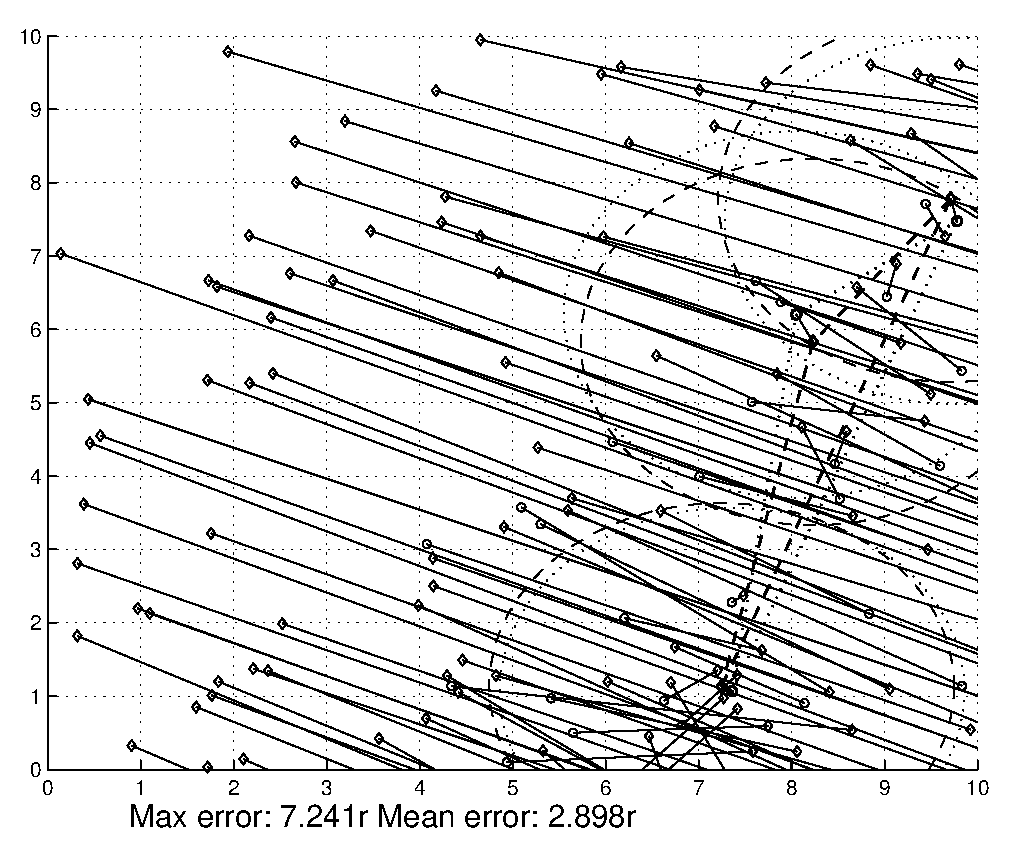
\includegraphics[width=\figurewidth\textwidth]{outliers/AS6/AS6NetworkDiff9}}
\\
	\subfloat[A normal network difference]{\label{fig:normal1}
		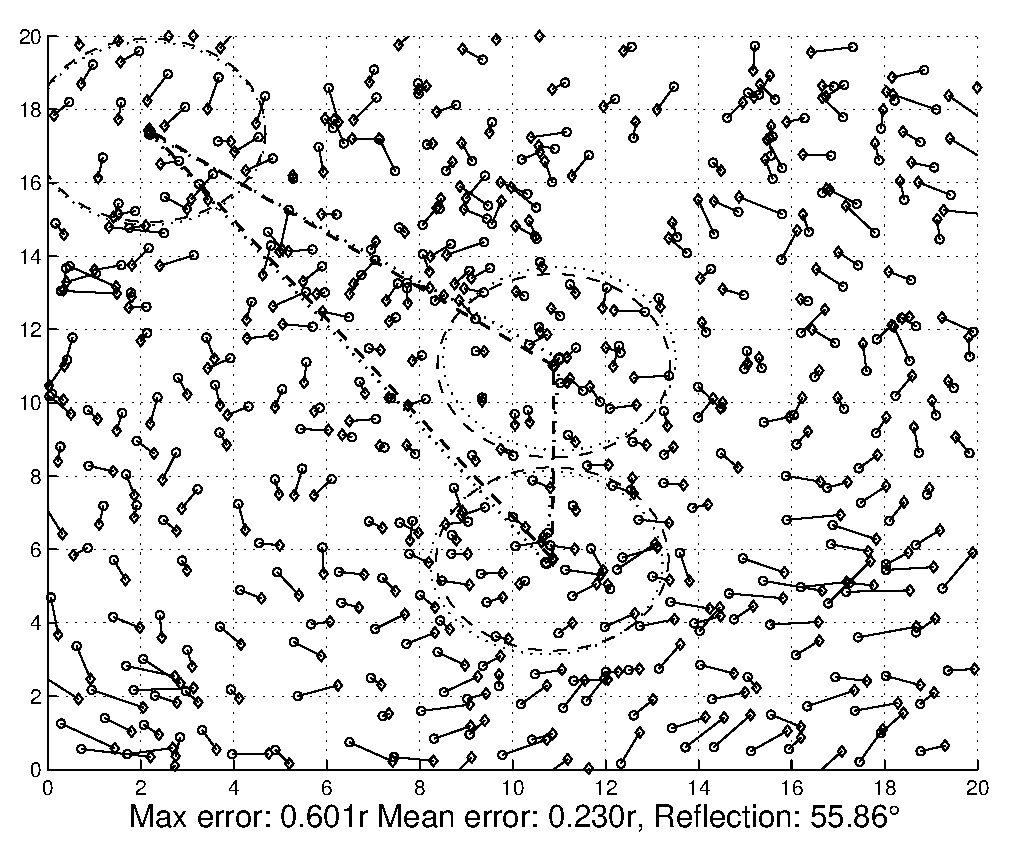
\includegraphics[width=\figurewidth\textwidth]{outliers/normal1}}		
	\label{fig:outliernetworkdiff}
	\caption{Network map of localization performance at each node}
\end{figure}

\subsection{Transformation Reflection and Rotation}
\label{sec:reflection}
Unfortunately, simply disabling the reflection component of the Procrustes transformation algorithm does not solve the problem.  The output of the Procrustes algorithm is a linear transformation which includes a rotation or reflection matrix, as discussed in Section~\ref{sec:procrustes}.  If the determinant of that matrix is +1, then the resulting transformation has a rotation, with an angle as in Equation~\ref{eqn:rotmatrix}.  

\begin{equation}
	\det{(T)}=+1 \Rightarrow ~Rotation ~with ~T=
	\begin{bmatrix}
	\cos{\theta} & -\sin{\theta} \\ 
	\sin{\theta} & \cos{\theta}\end{bmatrix}
	\label{eqn:rotmatrix} 
\end{equation}

If the determinant is -1, then the resulting transformation has a reflection component across a line at an angle as shown in Equation~\ref{eqn:refmatrix}. 

\begin{equation}
	\det{(T)}=-1 \Rightarrow ~Reflection ~with ~T=
	\begin{bmatrix}
	\cos{2{\theta}} & \sin{2{\theta}} \\ 
	\sin{2{\theta}} & -\cos{2{\theta}}\end{bmatrix}
	\label{eqn:refmatrix} 
\end{equation}

Figure~\ref{fig:rotref} shows the rotation and reflection distributions of two different networks, for a random set of anchor sets for each network.  In both networks, and with consistency across others, the bulk of the data points have the same angle of either rotation or reflection, while the outliers have the opposite property with a wide variance in the angle.  However, in different networks, it is not consistently either rotation or reflection that leads to poor localization results.  Therefore, relying on the determinant of the transformation is not a sufficient indicator for a network designer knowing that an outlier case has been detected and that the localization results are essentially useless.

\begin{figure}
  \centering
	\subfloat[A network where reflection is good]{\label{fig:rotref1}
		\includegraphics[width=\figurewidth\textwidth]{chapter5/a/RotRefvsError}}
\\
	\subfloat[A network where rotation is good]{\label{fig:rotref2}
		\includegraphics[width=\figurewidth\textwidth]{chapter5/b/RotRefvsError}}
	\caption{Rotation and reflection versus location error}	
	\label{fig:rotref}
\end{figure}

\subsection{Transformation Scaling and Translation}

For completeness, we explore the possibility that the scaling or translation component of the linear transformation is causing the issue.  In Figure~\ref{fig:scalar}, the scale component, \emph{b}, of the Procrustes analysis is plotted against the mean location error for the same two networks as shown above for reflection and rotation in Figure~\ref{fig:rotref}.  While there is an apex of the data around a particular scalar value where the minimum localization error is seen, the outliers can also have this same scalar value.  Therefore, the scaling component is not a good indicator of  extremely poor localization performance.

\begin{figure}
  \centering
	\subfloat[Corresponding to a network where reflection is good]{\label{fig:scalar1}
		\includegraphics[width=\figurewidth\textwidth]{chapter5/a/TransformScalar}}
\\
	\subfloat[Corresponding to a network where rotation is good]{\label{fig:scalar2}
		\includegraphics[width=\figurewidth\textwidth]{chapter5/b/TransformScalar}}
	\caption{Transformation scalar component versus location error}	
	\label{fig:scalar}
\end{figure}

Likewise, Figure~\ref{fig:translate} plots the horizontal, \emph{x}, and vertical, \emph{y}, translation components, \emph{c}, against the mean location error. As with the other transformation components, there is concentration around a \emph{natural} value in \emph{x} and \emph{y} that gives best localization performance.  The fact this value \emph{x} and \emph{y} overlap in Figure~\ref{fig:translate1} is a coincidence. However, much like for the scaling factor, while outlier localization errors are the only values that occur away from this natural value, the outliers also occur around that value as well.  Therefore, it is not possible to classify an anchor set as one of the outlier cases based on the translation component of the linear transformation it produces.

\begin{figure}
  \centering
	\subfloat[Corresponding to a network where reflection is good]{\label{fig:translate1}
		\includegraphics[width=\figurewidth\textwidth]{chapter5/a/TransformTranslate}}
\\
	\subfloat[Corresponding to a network where rotation is good]{\label{fig:translate2}
		\includegraphics[width=\figurewidth\textwidth]{chapter5/b/TransformTranslate}}
	\caption{Transformation translation component versus location error}	
	\label{fig:translate}
\end{figure}

\subsection{Procrustes Dissimilarity}

The Procrustes algorithm itself provides a measure of the dissimilarity.  Specifically, it is the minimized value of sum of squared errors\cite{procrustes-matlab}.  As shown in Figure~\ref{fig:dissimilarity}, it is not a good indicator of the transformation as it pertains to the entire network.  This is because the Procrustes algorithm is only performed on the anchor nodes themselves and for those nodes themselves, the transformation is good.

\begin{figure}
  \centering
	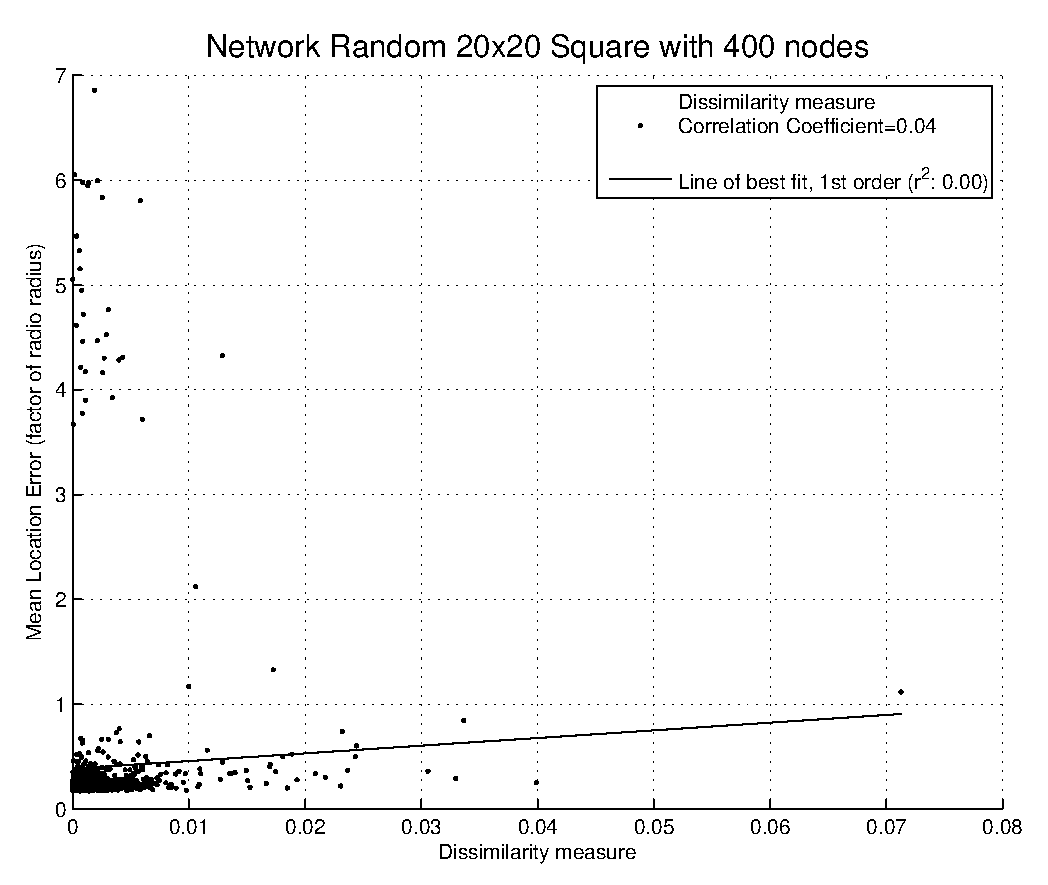
\includegraphics[width=\textwidth]{dissimilarity}
	\caption{Procrustes dissimilarity measure}	
	\label{fig:dissimilarity}
\end{figure}

\section{Outlier Indicators} 
\label{sec:outlierindicators}
As shown above, there unfortunately is no direct indicator that a particular anchor set generates a transformation with an incorrect angle.  Therefore, network designers must avoid all anchor sets that could potentially generate such an angle.  As demonstrated in Section~\ref{sec:anchorTriangle}, the area or height of the triangle formed by the anchor nodes is a good indicator of the possibility of a poor transformation angle.  These two metrics are explored in Figures~\ref{fig:heightIndicator} and \ref{fig:areaIndicator}, respectively.  This time, the x-axis is a log scale to better show the outlier cases. Also, the area and height itself has been adjusted as a factor of radius. Further, 95\% confidence intervals are shown for the mean of each 0.1r increment of both area and height.  A solid horizontal line is shown throw each mean, indicating the width of the increment, since it can be difficult to visualize on a log scale.  As the area and height increase, the mean expected area and height decrease, as does the confidence interval of that mean.  The horizontal dashed line indicates the cutoff for what are considered outliers, based on the large gap in data points.  The vertical dashed line indicates the first interval in which there are no outliers.  

\begin{figure}
  \centering
	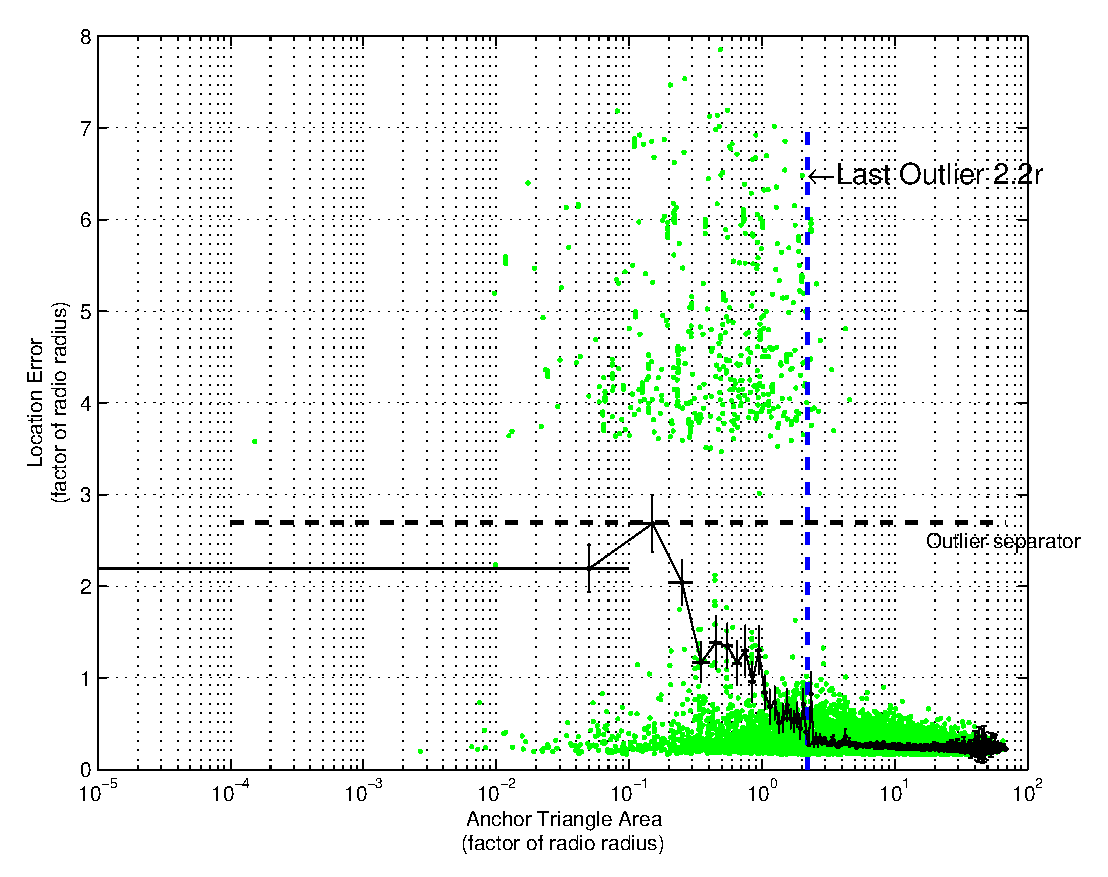
\includegraphics[width=\textwidth]{AreaIndicator_square}
	\caption[Anchor triangle areas]{Anchor triangle areas, with confidence intervals grouped in intervals of 0.1r}	
	\label{fig:areaIndicator}
\end{figure}

\begin{figure}
  \centering
	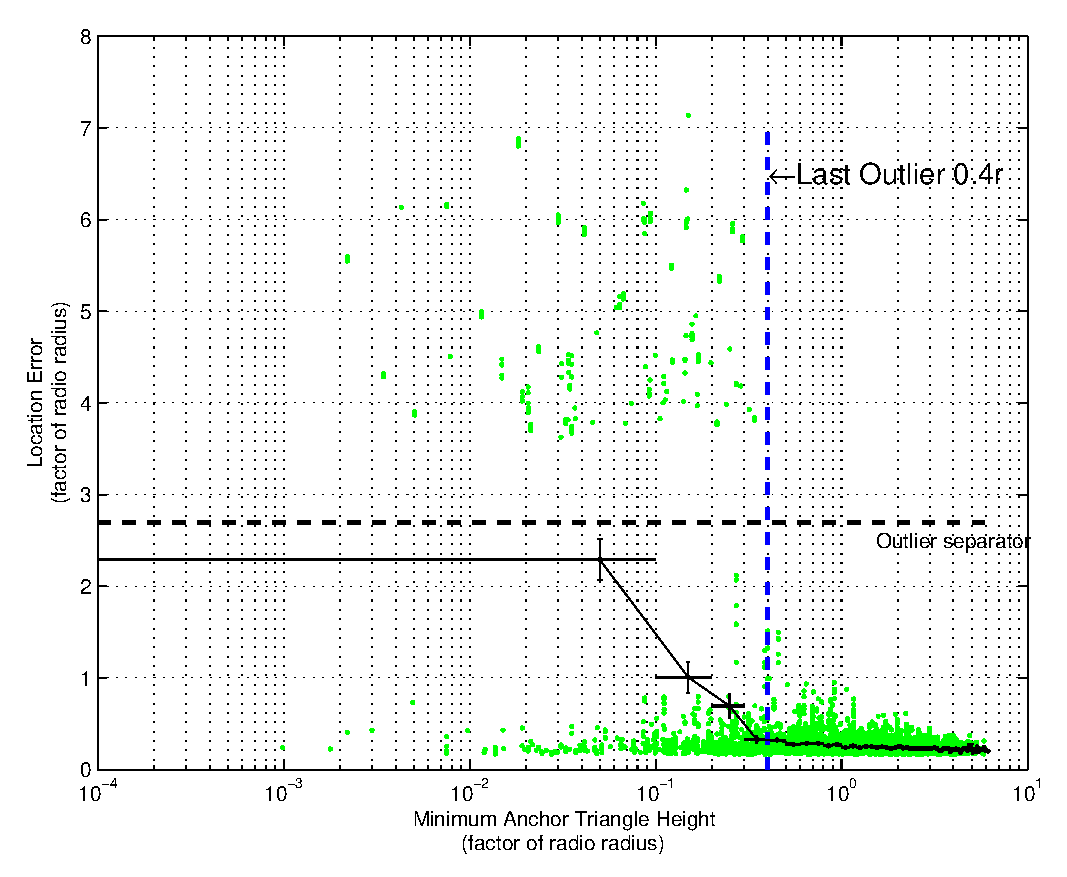
\includegraphics[width=\textwidth]{HeightIndicator_square}
	\caption[Minimum anchor triangle heights]{Minimum anchor triangle heights, with confidence intervals grouped in intervals of 0.1r}	
	\label{fig:heightIndicator}
\end{figure}

Upon comparing the two plots, it is clear that the minimum height metric is far more stable when it comes to predicting outliers than the area metric.  This is based on the observation that the mean localization error monotonically decreases with increased minimum height, while the mean localization error relative to area is far more erratic.  Further, there are some outlier cases after the first interval of triangle area that has no outliers.  A triangle with small area might provide a false-positive indication of an outlier.  After careful thought, this result is not unexpected since height of a triangle geometrically exposes collinearity better than simply area of a triangle.

Based on the minimum height statistics, we can now give network designers a metric of how collinear is too collinear for a set of anchor nodes.  The raw statistics indicate that if the triangle formed by the anchor nodes has a minimum height greater that 0.6 times the radio range, then there is very low probability of getting an extreme outlier case were the calculated locations are actually reflected or rotated across the network.  However, also in the data shown, there are some near-outlier cases beyond this point.  While these cases are not of the extreme nature discussed, it it worthwhile to give a margin of error here to avoid these cases as well.  Therefore, we assert that the triangle formed by the anchor nodes should have a minimum height equal to the radio range of the network.
